\subsection{The Memory Layout of an SGX Enclave}
\label{sec:sgx_enclave_layout}

SGX was designed to minimize the effort required to convert application code to
take advantage of enclaves. History suggests this is a wise decision, as a
large factor in the continued dominance of the Intel architecture is its
ability to maintain backward compatibility. To this end, SGX enclaves were
designed to be conceptually similar to the leading software modularization
construct, dynamically loaded libraries, which are packaged as \texttt{.so}
files on Unix, and \texttt{.dll} files on Windows.


\subsubsection{The Enclave Linear Address Range (ELRANGE)}
\label{sec:sgx_elrange}

% SGX Enclave Control Structure (SECS): SDM S 38.7

Each enclave designates an area in its virtual address space, called the
\textit{enclave linear address range} (ELRANGE), which is used to map the code
and the sensitive data stored in the enclave's EPC pages. The virtual address
space outside ELRANGE is mapped to access non-EPC memory via the same virtual
addresses as the enclave's host application, as shown in
Figure~\ref{fig:sgx_elrange}.

\begin{figure}[hbt]
  \centering
  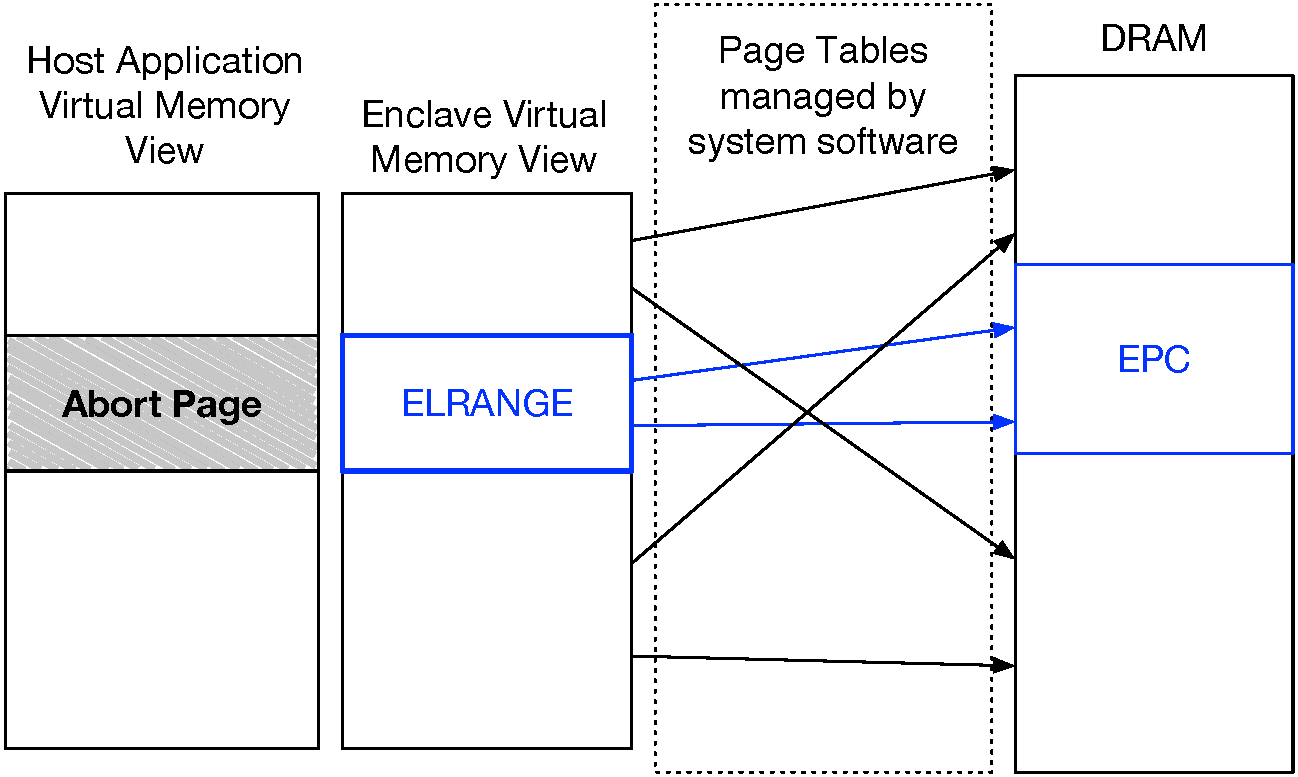
\includegraphics[width=85mm]{figures/sgx_elrange.pdf}
  \caption{
    An enclave's EPC pages are accessed using a dedicated region in the
    enclave's virtual address space, called ELRANGE. The rest of the virtual
    address space is used to access the host application's memory. The memory
    mappings are established using the page tables managed by system software.
  }
  \label{fig:sgx_elrange}
\end{figure}

The word ``linear'' in ELRANGE references the linear addresses produced by the
vestigial segmentation feature~(\S~\ref{sec:segments}) in the 64-bit Intel
architecture. For most purposes, ``linear'' can be treated as a synonym for
``virtual''.

ELRANGE is specified using a base (the BASEADDR field) and a size (the SIZE)
in the enclave's SECS~(\S~\ref{sec:sgx_secs}). ELRANGE must meet the same
constraints as a variable memory type range (\S~\ref{sec:cacheability_config})
and as the PRM range~(\S~\ref{sec:sgx_prm}), namely the size must be a power of
2, and the base must be aligned to the size. The main benefit of these
restrictions is that checking whether an address belongs to an enclave's
ELRANGE can be done very inexpensively in either
hardware~(\S~\ref{sec:cacheability_config}) or software.

When an enclave represents a dynamic library, it is natural to have ELRANGE be
set to the memory range reserved for the library by the loader. The ability to
access non-enclave memory from enclave code makes it easy to reuse existing
library code that expects to receive pointers to memory buffers managed by
the host application, and reads or modifies the buffers.


\subsubsection{Address Translation for SGX Enclaves}
\label{sec:sgx_paging}

% Access Control Requirements: SDM S 38.3
% Interactions with VMX: SDM S 42.5, S 42.5.{1,2,3,4,5}

Under SGX, the operating system and hypervisor are still in full control of the
page tables and EPTs, and each enclave's code uses the same address translation
process and page tables~(\S~\ref{sec:paging}) as its host application. This
minimizes the amount of changes required to add SGX support to existing system
software. At the same time, having the page tables managed by untrusted system
software opens up SGX to the address translation attacks described in
\S~\ref{sec:paging_attacks}. As future sections will reveal, a good amount of
the complexity in SGX's design can be attributed to the need to prevent these
address translation attacks.

SGX's active memory mapping attacks defense mechanisms revolve around ensuring
that each EPC page can only be mapped at a specific virtual
address~(\S~\ref{sec:segments}). When an EPC page is allocated, its intended
virtual address is recorded in the EPCM entry for the page, in the ADDRESS
field.

When an address translation (\S~\ref{sec:paging}) result is the physical
address of an EPC page, the CPU ensures\footnote{A mismatch triggers a general
protection fault (\#GP, \S~\ref{sec:faults}).} that the virtual address given
to the address translation process matches the expected virtual address
recorded in the page's EPCM entry.

SGX also prevents against some passive memory mapping attacks and fault
injection attacks by ensuring that the access permissions of each EPC page
always match the enclave author's intentions. The access permissions for each
EPC page are specified when the page is allocated, and recorded in the
\textit{readable}~(R), \textit{writable}~(W), and \textit{executable}~(X)
fields in the page's EPCM entry, shown in
Table~\ref{fig:sgx_epcm_access_fields}.

\begin{table}[hbt]
  \centering
  \begin{tabularx}{\columnwidth}{| l | r | X |}
  \hline
  \textbf{Field} & \textbf{Bits} & \textbf{Description}\\
  \hline
  ADDRESS & 48 & the virtual address used to access this page\\
  \hline
  R & 1 & allow reads by enclave code\\
  \hline
  W & 1 & allow writes by enclave code\\
  \hline
  X & 1 & allow execution of code inside the page, inside enclave\\
  \hline
  \end{tabularx}
  \caption{
    The fields in an EPCM entry that indicate the enclave's intended virtual
    memory layout.
  }
  \label{fig:sgx_epcm_access_fields}
\end{table}

When an address translation (\S~\ref{sec:paging}) resolves into an EPC page,
the corresponding EPCM entry's fields override the access permission attributes
(\S~\ref{sec:page_table_attributes}) specified in the page tables. For example,
the W field in the EPCM entry overrides the writable (W) attribute, and the X
field overrides the disable execution (XD) attribute.


It follows that an enclave author must include memory layout information along
with the enclave, in such a way that the system software loading the enclave
will know the expected virtual memory address and access permissions for each
enclave page. In return, the SGX design guarantees to the enclave authors that
the system software, which manages the page tables and EPT, will not be able to
set up an enclave's virtual address space in a manner that is inconsistent with
the author's expectations.

The \texttt{.so} and \texttt{.dll} file formats, which are SGX's intended
enclave delivery vehicles, already have provisions for specifying the virtual
addresses that a software module was designed to use, as well as the desired
access permissions for each of the module's memory areas.


\subsubsection{The Thread Control Structure (TCS)}
\label{sec:sgx_tcs}

% Thread Control Structure (TCS): SDM S 38.8, S 38.8.{1,2,3,4}

The SGX design fully embraces multi-core processors. It is possible for
multiple logical processors~(\S~\ref{sec:cpu_die}) to concurrently execute the
same enclave's code at the same time, via different threads.

The SGX implementation uses a \textit{Thread Control Structure}~(TCS) for each
logical processor that executes an enclave's code. It follows that an enclave's
author must provision at least as many TCS instances as the maximum number of
concurrent threads that the enclave is intended to support.

Each TCS is stored in a dedicated EPC page whose EPCM entry type is PT\_TCS.
The SDM describes the first few fields in the TCS. These fields are considered
to belong to the architectural part of the structure, and therefore are
guaranteed to have the same semantics on all the processors that support SGX.
The rest of the TCS is not documented.

% Access Control Requirements: SDM S 38.3
% EDBGRD, EDBGWR: SDM S 41.3

The contents of an EPC page that holds a TCS cannot be directly accessed, even
by the code of the enclave who owns the TCS. This restriction is similar to the
restriction on accessing EPC pages holding SECS instances. However, the
architectural fields in a TCS can be read by enclave debugging instructions.

The architectural fields in the TCS layout  the context
switches~(\S~\ref{sec:registers}) performed by a logical processor when it
transitions between executing non-enclave and enclave code.

For example, the OENTRY field specified the value loaded in the instruction
pointer (RIP) when the TCS is used to start executing enclave code, so the
enclave author has strict control over the entry points available to enclave's
host application. Furthermore, the OFSBASGX and OFSBASGX fields specify the
base addresses loaded in the FS and GS segment
registers~(\S~\ref{sec:segments}), which typically point to Thread Local
Storage (TLS).


\subsubsection{The State Save Area (SSA)}
\label{sec:sgx_ssa}

% State Save Area (SSA) Frame: SDM S 38.9

When the processor encounters a hardware exception~(\S~\ref{sec:faults}), such
as an interrupt~(\S~\ref{sec:interrupts}), while executing the code inside an
enclave, it performs a privilege level switch (\S~\ref{sec:faults}) and invokes
a hardware exception handler provided by the system software. Before executing
the exception handler, however, the processor needs a secure area to store the
enclave code's execution context~(\S~\ref{sec:registers}), so that the
information in the execution context is not revealed to the untrusted system
software.

% SECS.SSAFRAMESIZE: SDM S 42.7.2.2

In the SGX design, the area used to store an enclave thread's execution context
while a hardware exception is handled is called a \texttt{State Save
Area}~(SSA), illustrated in Figure~\ref{fig:sgx_enclave_layout}. Each TCS
references a contiguous sequence of SSAs. The OSSA field specifies the location
of the first SSA in the enclave's virtual address space, and the NSSA field
indicates the number of available SSAs. Each SSA starts at the beginning of an
EPC page, and uses up the number of EPC pages that is specified in the
SSAFRAMESIZE field of the enclave's SECS.

\begin{figure}[hbt]
  \centering
  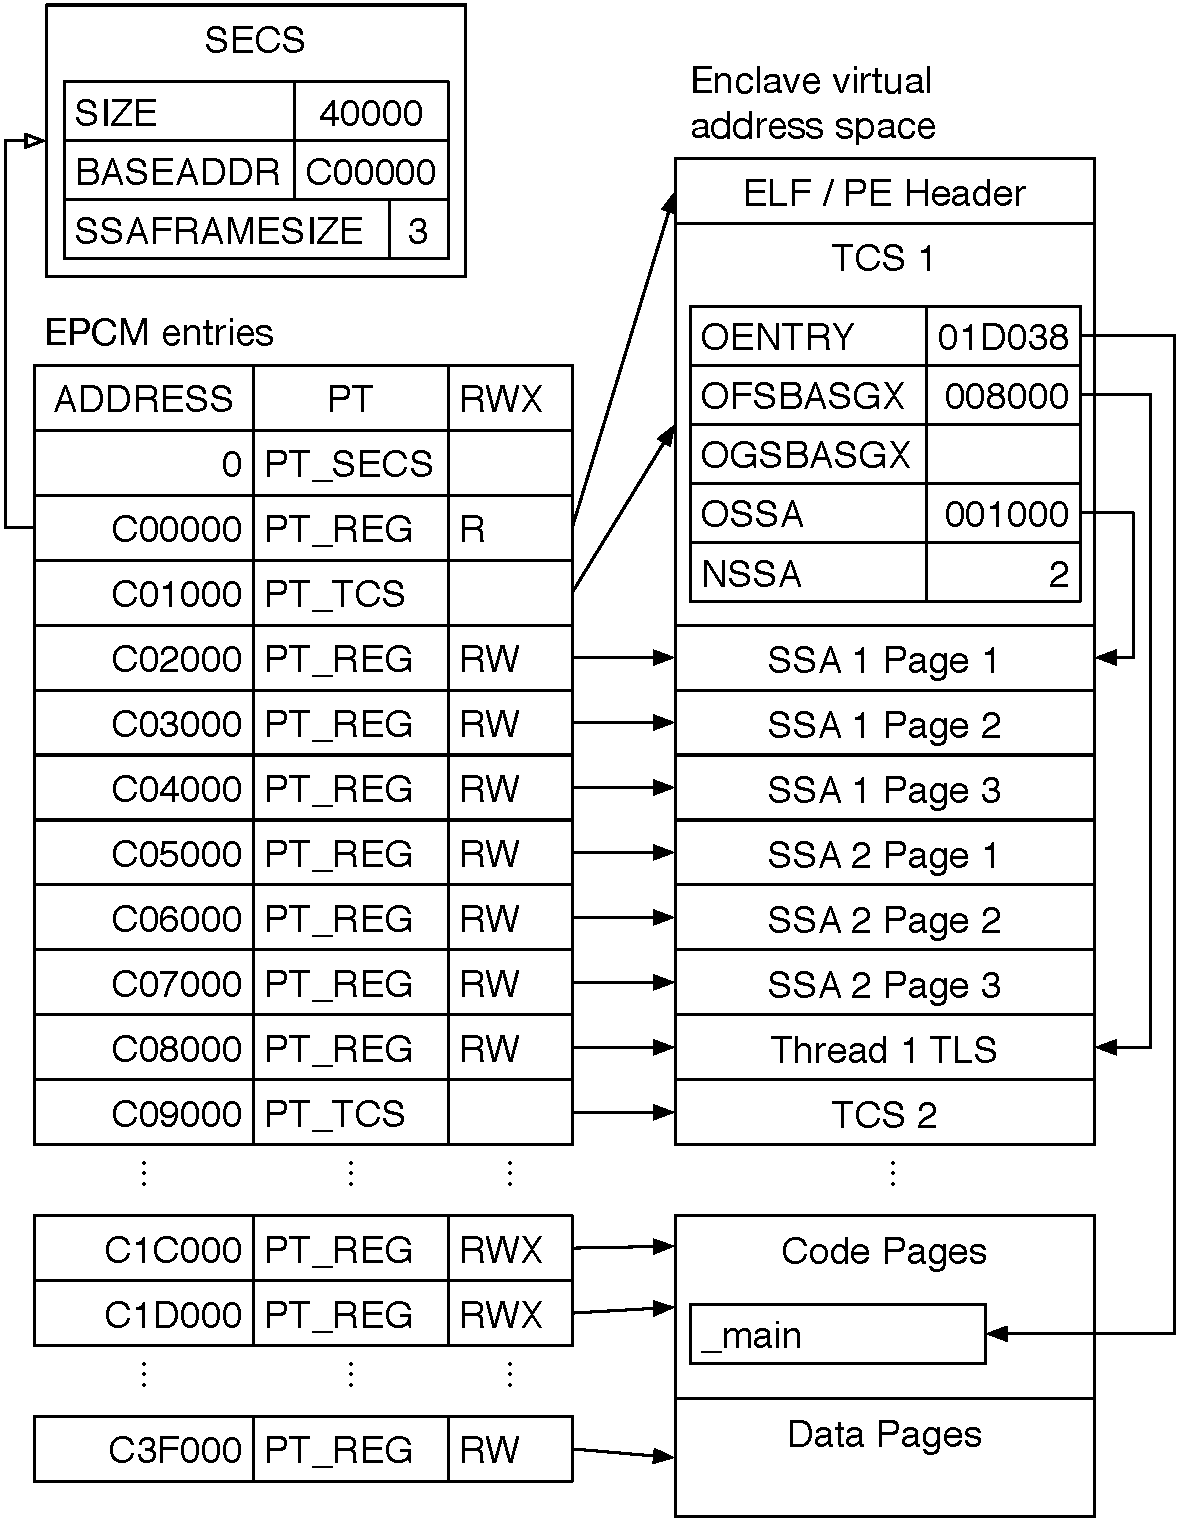
\includegraphics[width=85mm]{figures/sgx_enclave_layout.pdf}
  \caption{
    A possible layout of an enclave's virtual address space. Each enclave has a
    SECS, and one TCS per supported concurrent thread. Each TCS points to a
    sequence of SSAs, and specifies initial values for RIP and for the base
    addresses of FS and GS.
  }
  \label{fig:sgx_enclave_layout}
\end{figure}

An enclave thread's execution context consists of the general-purpose registers
(GPRs) and the result of the XSAVE instruction~(\S~\ref{sec:registers}).
Therefore, the size of the execution context depends on the requested-feature
bitmap~(RFBM) used by to XSAVE. All the code in an enclave uses the same RFBM,
which is declared in the XFRM sub-field of the ATTRIBUTES field of the
enclave's SECS. The number of EPC pages reserved for each SSA, specified in
SSAFRAMESIZE, must\footnote{\texttt{ECREATE}~(\S~\ref{sec:sgx_ecreate}) fails
if SSAFRAMESIZE is too small.} be large enough to fit the XSAVE output for the
feature bitmap specified in XFRM.

SSAs are stored in regular EPC pages, whose EPCM page type is PT\_REG.
Therefore, the SSA contents is accessible to enclave software. The SSA layout
is architectural, and is completely documented in the SDM. This opens up
possibilities for an enclave exception handler that is invoked by the host
application after a hardware execption occurs, and acts upon the information in
a SSA.
